\documentclass{homework}
\author{Haley Beauchamp, Ryan Seaman}
\class{CSCI 4063: Senior Capstone (Tashfeen)}
\date{10 October 2025}
\title{Proposal}
\address{%
  Oklahoma City University, %
  Petree College of Arts \& Sciences, %
  Computer Science%
}

\acmfonts

\usepackage{graphicx}

\begin{document} \maketitle

\textbf{Description:} 

A cross-platform mobile app that recommends posts to users based on their progress in a tv series to avoid spoilers and promote a safe fandom experience. It will have a simple UI similar to Tumblr, where users can read and write text-based posts about fandoms they enjoy. We will implement \hyperref[explanation]{Retrieval-Augmented Generation} to flag spoilers and improve the user experience. 

\bigskip

\textbf{Libraries:}
\begin{itemize}
  \item Frontend: 
  \href{https://flutter.dev/}{Flutter}, \href{https://dart.dev/}{Dart}
  \item Backend:    \href{https://expressjs.com/}{Express}, \href{https://www.typescriptlang.org/}{TypeScript}, 
  \href{https://nodejs.org/en}{Node}
  \item LLM: 
  \href{https://openai.com/}{OpenAI}
  \item Database: 
  \href{https://typeorm.io/}{TypeORM}, \href{https://www.postgresql.org/}{PostgreSQL}, hosted by
  \href{https://neon.com/}{Neon}
  \item Containerization: \href{https://www.docker.com/}{Docker}
\end{itemize}

\bigskip

\textbf{Features:}
\begin{itemize}
  \item User accounts and authentication
  \item Text-based UI similar to Tumblr

  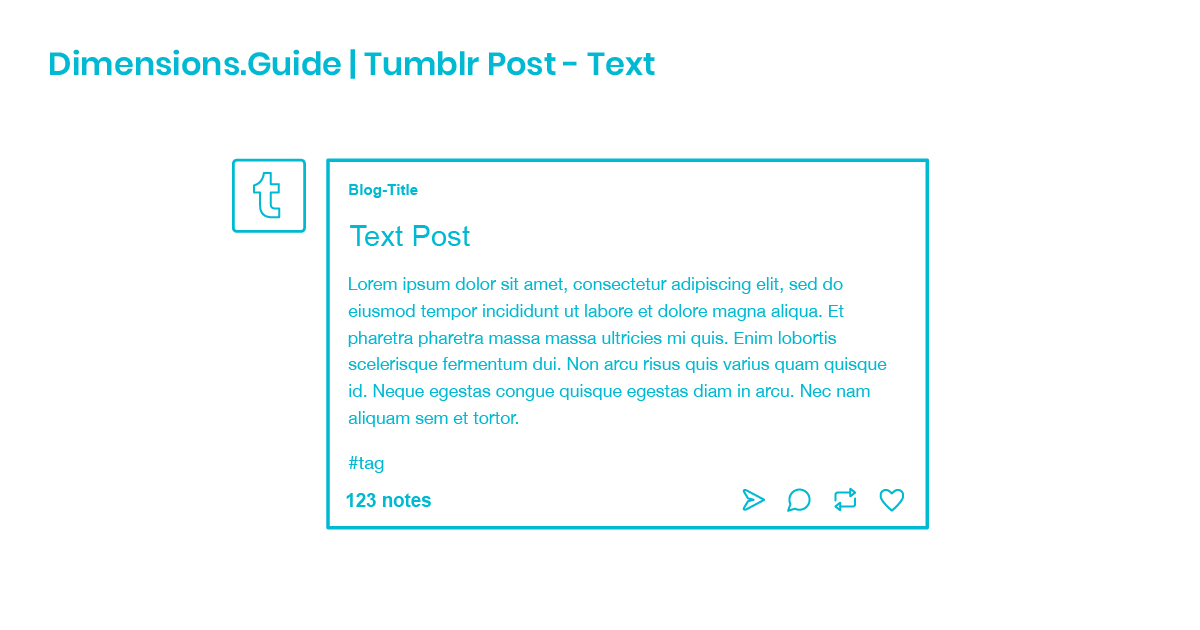
\includegraphics[width=0.8\textwidth]{media/tumblr_example.jpg}

  \item Ability to input your current episode for a given tv show
  \item Recommendation of posts based on current episode in a series - spoiler control, tagging system
  \item Post interactions like liking and commenting
  \item User following system
  \item User customization like profile pictures
\end{itemize}

\bigskip

\textbf{Stretch Goals:}
\begin{itemize}
  \item Support for multimedia posts (images, videos)
  \item Support for media types beyond tv shows (movies, games)
  \item Enhanced profile customization (themes, advanced layouts)
\end{itemize}

\bigskip

\label{explanation} \textbf{Retrieval Augmented Generation}

Retrieval-Augmented Generation is a method of allowing llms to respond to queries using supporting information beyond their training data. 

Our implementation will involve retrieving relevant transcript data from a database to inform llm spoiler detection.

% \newpage
% \bibliographystyle{plain}
% \bibliography{citations}
\end{document}
